\section{Programmiermodel}
In diesem Kapitel wird sich der Konzeption eines Programmiermodells auf Basis der Anforderungen (insbesondere NFN\#0) und der Entscheidungen aus dem vorhergegangenen Kapitel konzeptioniert.

\subsection{Datenfluss-basierte Programmierung}\label{subsection:datenflussprog}
Wie in Kapitel \ref{subsec:characIot} geschrieben sind Prototypen, die mit cBlocks entwickelt werden essentiell einem Netzwerk von Sensoren, welche Daten versenden, diese in eine nutzbare Form verwandeln und von Aktoren konsumiert werden. Diese Form von Signal-Kommunikation ist ähnlich derer von \ac{DBP}. Die Definition  laut \cite{sousa2012dataflow} von \ac{DBP} ist:
\begin{quote}
    '' \textit{Die Programmierung anhand von Datenflüssen führt ein ein neues Paradigma ein, bei dem die interne Struktur eines Programmes mit einem gerichteten Graphen repräsentiert wird, ähnlich wie bei einem Datenflussdiagramm.} ''
\end{quote}

\begin{figure}[h]
\centering
\begin{subfigure}{.45\textwidth}
  \centering
  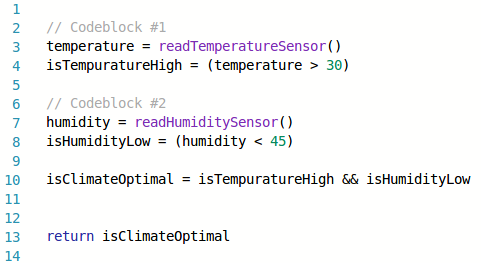
\includegraphics[width=1\linewidth]{bilder/chapter4/chapter4_2/codekbpbeispiel.png}
  \caption{}
  \label{fig:subvgldbptexttext}
\end{subfigure}%
\begin{subfigure}{.55\textwidth}
  \centering
  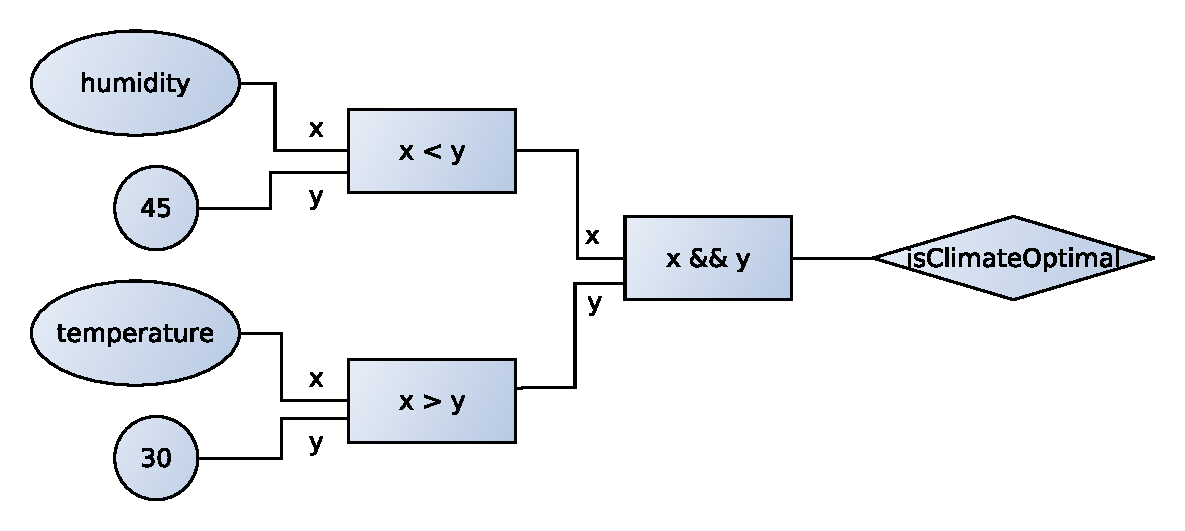
\includegraphics[width=1\linewidth]{bilder/chapter4/chapter4_2/beispieldatenfluss.pdf}
  \caption{}
  \label{fig:subvgldbptextdbp}
\end{subfigure}
    \caption{Der gleiche Programmcode in zwei Ansichten: \ac{KBP} (a) und \ac{DBP} (b). Hierbei ist die sequentielle Durchführung des \ac{KBP}-Modells mit der Parallelen des \ac{DBP} erkenntlich. Während beim linken Paradigma sequentiell die Blöcke abgearbeitet werden (wobei \#1 fertig sein muss um \#2 zu berechnen), ist das rechte Paradigma unabhängig von der Reihenfolge, in der die Signale eintreffen. Dies spiegelt den asynchronen Sachverhalt von \ac{WSAN} wieder.}
    \label{fig:bfd}
\end{figure}


Ein solches Programm wird in Abbildung \ref{fig:bfd} veranschaulicht. In dem konkreten Graphen handelt es sich um ein typisches Szenario, wie es mit flowws modelliert werden kann. Der Kontrollfluss-basierte Pseudocode zum selben Programm ist daneben zu sehen. In der Darstellung können vier verschiedene Elemente ausgemacht werden, die den Datenflussgraphen ausmachen. Die einzelnen Elemente, die mit dem Domänenmodel (Abbildung \ref{fig:bfddomainmodel}) korrespondieren sind:
\begin{figure}[h]
  \centering
  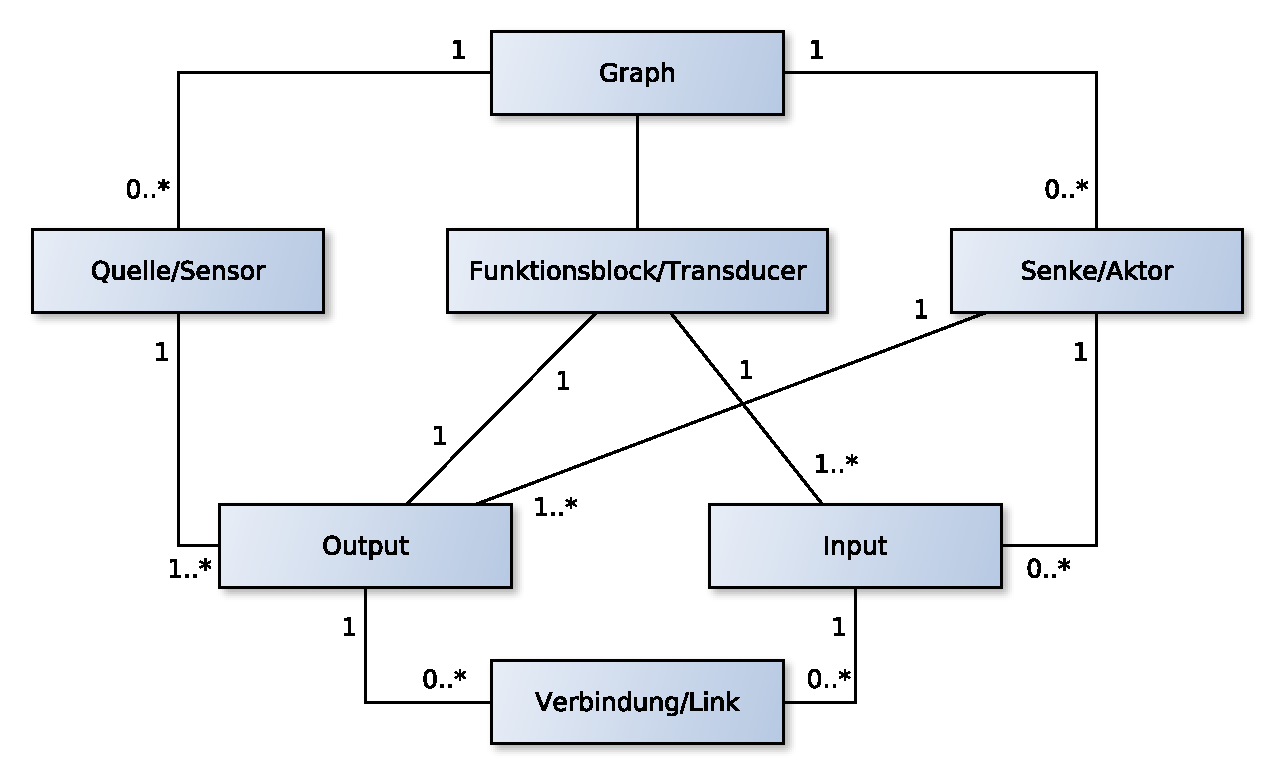
\includegraphics[width=0.75\textwidth]{bilder/chapter4/chapter4_2/domainmodelldatenfluss.pdf}
  \caption{Das Domänenmodell des eines Datenflussprogrammes (in flowws) besteht aus drei Sorten von Knoten: Quellen/Sensoren, Senken/Aktoren und Funktionsblöcke/Transducer. Sie besitzen (mit Ausnahme der Quelle) Output- und Input-Interfaces, die es den Knoten erlauben durch Verbindungen/Links zu kommunizieren}
  \label{fig:bfddomainmodel}
\end{figure}
\begin{itemize}
    \item \textbf{Quellen} erzeugen die zu verarbeitenden Daten. Innerhalb von flowws bzw. cBlocks Netzwerken werden (virtuelle) Konstanten und (physische) Sensoren als datenerzeugendende Quellen angesehen. 
    \item \textbf{Funktionsblöcke} verarbeitenden Daten. Jeder Funktionsblock ist eine \textit{Black Box}, die aus einer Anzahl von Input-/Output-Schnittstellen und einer Verarbeitungslogik bestehen. Die Verarbeitungslogik wird im Falle von flowws von den funktionellen Anforderungen FA\#1 bis FA\#6 (Kapitel \ref{subsec:fanf}) vorgegeben. Nicht nur die Transformationen von Daten aber auch temporale Operationen wie die zeitliche Verzögerung eines Signals werden in diesen Blöcken abgearbeitet. 
    \item \textbf{Senken} konsumieren die erzeugten/verarbeitenden Daten. Innerhalb von flowws bzw. cBlocks Netzwerken übernehmen (virtuelle) Schnittstellen zu (physischen) Aktoren diese Aufgabe. Sie verwenden die erzeugten Daten um ein bestimmtes Verhalten in Aktoren innerhalb des Systems herbeizuführen.
    \item \textbf{Verbindungen} transferieren Signale bzw. Nachrichten zwischen den Knotenpunkten. Sie definieren die eins-zu-eins Verbindung zwischen den Input/Output-Schnittstellen der Funktionsblöcke. Diese Verbindung ist gerichtet d.h. Daten fließen immer nur in eine Richtung durch den Graphen.
    \item \textbf{Ereignisse} sind Nachrichten, die durch das Netzwerk von Node zu Node fließen. Sie beinhalten neben einem \textit{Payload}, der die eigentlichen Daten besitzt, auf dem die Transformationen durchgeführt werden, noch zusätzliche Metainformationen, die für die Bearbeitung der Daten wichtig sind. Die Datentypen, die der \textit{Payload} in besitzen kann wird von cBlocks-Ökosystem festgelegt und kann in Tabelle \ref{tab:datentypenpayloads} nachgelesen werden.
\end{itemize}

 \begin{table}[h]
\caption{Die drei verschiedenen Datentypen von Ereignis-\textit{Payloads}, die innerhalb von flowws verwendet werden.}
\label{tab:datentypenpayloads}
\begin{tabularx}{\textwidth}{llXX}
\hline
\rowcolor[HTML]{EFEFEF} 
Datentyp & Beispiel &  Erläuterung &  Verwendung \\ \hline
Number & 0,1,2,3.43,-12...& nummerischer Wert (Ganzzahlig und Fließkomma) & Temperatur, Abstand, Helligkeit, ...   \\ \hline
String & "qwnTZ32" & beliebige Zeichenkette & RFID-Code, Farbcodes, Display-Text, ... \\ \hline
Boolean & true, false & Wahrheitswert & Taster, Relays, ... \\ \hline
\end{tabularx}
\end{table}

\ac{DBP} erlaubt uns effizient die Komplexität von parallelen \textit{Events} zu modellieren und auch für nicht Experten zu visualisieren. Dies ist somit ein guter Anforderungen um die Anforderungen NFN\#2 und NFN\#0 zu erfüllen. Um NFN\#0 allerdings komplett zu erfüllen, muss ein weiterer Sachverhalt addressiert werden: das modellieren sequentieller Logik, wie sie in Problem ''Parallel contra Sequentiell'' beschrieben und in Szenario S\#2 verdeutlicht ist.